% ------------------------------------------------------------------------------
% TYPO3 CMS 8.3 - What's New - Chapter "In-Depth Changes" (English Version)
%
% @author	Patrick Lobacher <patrick@lobacher.de> and Michael Schams <schams.net>
% @license	Creative Commons BY-NC-SA 3.0
% @link		http://typo3.org/download/release-notes/whats-new/
% @language	English
% ------------------------------------------------------------------------------
% LTXE-CHAPTER-UID:		5ebcecbe-66abfa57-cf38bc00-aa637965
% LTXE-CHAPTER-NAME:	In-Depth Changes
% ------------------------------------------------------------------------------

\section{Modifiche rilevanti}
\begin{frame}[fragile]
	\frametitle{Modifiche rilevanti}

	\begin{center}\huge{Capitolo 3:}\end{center}
	\begin{center}\huge{\color{typo3darkgrey}\textbf{Modifiche rilevanti}}\end{center}

\end{frame}

% ------------------------------------------------------------------------------
% LTXE-SLIDE-START
% LTXE-SLIDE-UID:		7fdc3465-2d8b0c3a-e9de9a37-273fdb2c
% LTXE-SLIDE-ORIGIN:	bd33b29d-c20d1765-f923f78e-43bfb0bf English
% LTXE-SLIDE-TITLE:		Feature #74365: Add Linkservice for Unified Referencing Syntax (1)
% LTXE-SLIDE-REFERENCE:	Feature-74365-LinkServiceForUnifiedReferencingSyntax.rst
% ------------------------------------------------------------------------------
\begin{frame}[fragile]
	\frametitle{Modifiche rilevanti}
	\framesubtitle{Aggiunto Linkservice per la sintassi di Unified Referencing (1)}

	\begin{itemize}

		\item Nel passato le risorse in TYPO3 sono state referenziate in vari e differenti forme di sintassi.

		\item Ora TYPO3 supporta un moderno e futuristico modo di referenziare le risorse, una sintassi estendibile 
			facile da capire.

		\item Le slide sucessive spiegano la sintassi utilizzando il seguente link di pagina:

			\begin{lstlisting}
				t3://page?uid=13&campaignCode=ABC123
			\end{lstlisting}

	\end{itemize}

\end{frame}

% ------------------------------------------------------------------------------
% LTXE-SLIDE-START
% LTXE-SLIDE-UID:		f80015b5-5e552d0a-2a8da32d-d8e18fc0
% LTXE-SLIDE-ORIGIN:	95f9a663-ea2155a1-5635728b-77a8995c English
% LTXE-SLIDE-TITLE:		Feature #74365: Add Linkservice for Unified Referencing Syntax (2)
% LTXE-SLIDE-REFERENCE:	Feature-74365-LinkServiceForUnifiedReferencingSyntax.rst
% ------------------------------------------------------------------------------
\begin{frame}[fragile]
	\frametitle{Modifiche rilevanti}
	\framesubtitle{Aggiunto Linkservice per la sintassi di Unified Referencing (2)}

	\begin{itemize}

		\item La sintassi consiste in tre parti:

			\begin{itemize}

				\item Namespace (\texttt{t3://})\newline
		   			Il namespace è fissato a \texttt{t3://} al fine di garantire che "LinkService" venga eseguito per analizzare URN.
					\newline
				\item Chiave del gestore della risorsa (\texttt{page})\newline
   					La chiave del gestore della risorsa è uno della lista di gestori disponibili in TYPO3.
					Nel momento in cui si scrive esistono i seguenti gestori: \texttt{page}, \texttt{file} e \texttt{folder}.\newline
					Altre chiavi possono essere gestite in un array associativo, dove la chiave è il gestore e il valore
					è la classe che implementa LinkHandlerInterface:\newline
					\texttt{\$TYPO3\_CONF\_VARS['SYS']['linkHandler']}

			\end{itemize}

	\end{itemize}

\end{frame}

% ------------------------------------------------------------------------------
% LTXE-SLIDE-START
% LTXE-SLIDE-UID:		5261836d-6b54d631-b9a257ae-2f5e2280
% LTXE-SLIDE-ORIGIN:	77a8995c-ea2155a1-95f9a663-5635728b English
% LTXE-SLIDE-TITLE:		Feature #74365: Add Linkservice for Unified Referencing Syntax (3)
% LTXE-SLIDE-REFERENCE:	Feature-74365-LinkServiceForUnifiedReferencingSyntax.rst
% ------------------------------------------------------------------------------
\begin{frame}[fragile]
	\frametitle{Modifiche rilevanti}
	\framesubtitle{Aggiunto Linkservice per la sintassi di Unified Referencing (3)}

	\begin{itemize}

		\item ...e la terza parte:

			\begin{itemize}

				\item Parametri della risorsa (\texttt{?uid=13\&campaignCode=ABC123})\newline
					Questi sono i parametri identificativi specifici che sono utilizzati dal gestore.
					Si noti che essi possono riportare ulteriori parametri per configurare il comportamento in qualsiasi gestore.

			\end{itemize}

	\end{itemize}

\end{frame}

% ------------------------------------------------------------------------------
% LTXE-SLIDE-START
% LTXE-SLIDE-UID:		901d49db-8fe3ac1e-8e21cd62-1108e641
% LTXE-SLIDE-ORIGIN:	af8e73a4-2b315873-bb6e55e4-c0cd82b5 English
% LTXE-SLIDE-TITLE:		#76008 and #76458: DebuggerUtility::var_dump (1)
% LTXE-SLIDE-REFERENCE:	Feature-76008-PropertyVisibilityToDebuggerUtilityvar_dump.rst
% LTXE-SLIDE-REFERENCE:	Feature-76458-LetDebuggerUtilityRenderClosures.rst
% ------------------------------------------------------------------------------
\begin{frame}[fragile]
	\frametitle{Modifiche rilevanti}
	\framesubtitle{\texttt{DebuggerUtility::var\_dump} (1)}

	\begin{itemize}

		\item La visibilità dell'informazione strutturata è stata aggiunta a \texttt{DebuggerUtility::var\_dump()}
			\newline
			per ogni proprietà dell'oggetto in dump.

		\item Se una closure è parte dell'oggetto in debugging, anche il sorgente della closure verrà visualizzato.

	\end{itemize}

	\tabto{0.75cm}\textit{Vedi l'esempio nella slide seguente}

\end{frame}

% ------------------------------------------------------------------------------
% LTXE-SLIDE-START
% LTXE-SLIDE-UID:		bd7d3913-e68521e0-b7447db4-45170d40
% LTXE-SLIDE-ORIGIN:	bb6e55e4-2b315873-c0cd82b5-af8e73a4 English
% LTXE-SLIDE-TITLE:		#76008 and #76458: DebuggerUtility::var_dump (2)
% LTXE-SLIDE-REFERENCE:	Feature-76008-PropertyVisibilityToDebuggerUtilityvar_dump.rst
% LTXE-SLIDE-REFERENCE:	Feature-76458-LetDebuggerUtilityRenderClosures.rst
% ------------------------------------------------------------------------------
\begin{frame}[fragile]
	\frametitle{Modifiche rilevanti}
	\framesubtitle{\texttt{DebuggerUtility::var\_dump} (2)}

	\begin{figure}
		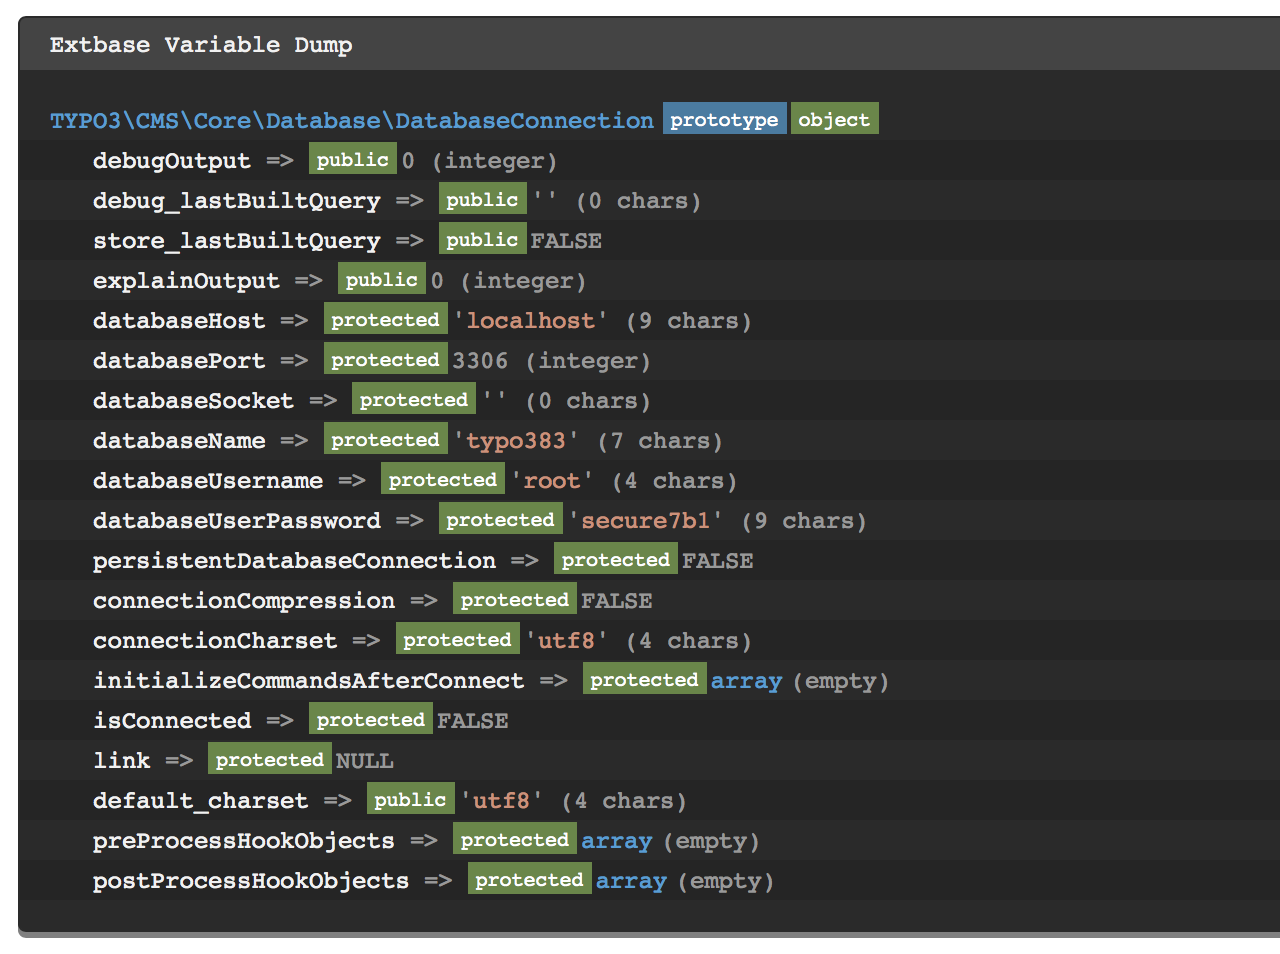
\includegraphics[width=0.65\linewidth]{InDepthChanges/76008.png}
	\end{figure}

\end{frame}

% ------------------------------------------------------------------------------
% LTXE-SLIDE-START
% LTXE-SLIDE-UID:		34046c6d-b97de7a2-e588ae5d-5d35e11c
% LTXE-SLIDE-ORIGIN:	2b74180d-e68ba0c2-8826a2cf-8498f977 English
% LTXE-SLIDE-TITLE:		!Breaking: #73461 - Import module disabled for non admin users
% LTXE-SLIDE-REFERENCE:	!Breaking-73461-ImportModuleDisabledForNonAdminUsers.rst
% ------------------------------------------------------------------------------
\begin{frame}[fragile]
	\frametitle{Modifiche rilevanti}
	\framesubtitle{Disabilitato il modulo di Import per gli utenti non Admin}

	\begin{itemize}

		\item Il modulo di import di \texttt{EXT:impexp} è ora disabilitato di default per gli utenti non amministratori

		\item Per gli utenti non amministratori, che necessitano di questa funzione, può essere usata la seguente opzione di 
			User TSconfig:\newline
			\texttt{options.impexp.enableImportForNonAdminUser = 1}

			\vspace{0.5cm}

			\begingroup
				\color{typo3red}
				Attenzione: questo potrebbe essere un problema di sicurezza nelle versioni di TYPO3 6.2 e 7.6,
				dovrebbe essere abilitato solo per \textit{affidabili} utenti di backend.
			\endgroup

	\end{itemize}

\end{frame}

% ------------------------------------------------------------------------------
% LTXE-SLIDE-START
% LTXE-SLIDE-UID:		a9054e5c-5898b8ca-75190959-01c9cba5
% LTXE-SLIDE-ORIGIN:	bac423cc-ba00db30-e1538b7f-25749380 English
% LTXE-SLIDE-TITLE:		Hooks and Signals (1)
% LTXE-SLIDE-REFERENCE:	!Feature-76209-HookToRegisterCustomResultBrowsersInAbstractPlugin.rst
% ------------------------------------------------------------------------------
\begin{frame}[fragile]
	\frametitle{Modifiche rilevanti}
	\framesubtitle{Hooks e Signals (1)}

	% decrease font size for code listing
	\lstset{basicstyle=\tiny\ttfamily}

	\begin{itemize}

		\item Un nuovo hook permette la registrazione di risultati personalizzati delle implementazioni di browser

		\item Questo approcio permette di ignorare l'implementazione predefinita di 
			\texttt{AbstractPlugin::pi\_list\_browseresults()}
			per tutte le estensioni o solo per specifiche estensioni

		\item L'hook può essere registrato in \texttt{ext\_localconf.php}:

			\begin{lstlisting}
				$GLOBALS['TYPO3_CONF_VARS']['SC_OPTIONS']
				  [\TYPO3\CMS\Frontend\Plugin\AbstractPlugin::class]['pi_list_browseresults'][1463475262] =
				  \Vendor\ExtensionKey\Hook\ResultBrowserHook::class
			\end{lstlisting}

	\end{itemize}

\end{frame}


% ------------------------------------------------------------------------------
% LTXE-SLIDE-START
% LTXE-SLIDE-UID:		4984aa08-08d141f2-e85841c6-13cbba80
% LTXE-SLIDE-ORIGIN:	82c70aee-3b375252-6cac0ad6-b385b95f English
% LTXE-SLIDE-TITLE:		Hooks and Signals (2)
% LTXE-SLIDE-REFERENCE:	!Feature-76259-IntroduceBuildQueryParametersPostProcessHook.rst
% ------------------------------------------------------------------------------
\begin{frame}[fragile]
	\frametitle{Modifiche rilevanti}
	\framesubtitle{Hooks e Signals (2)}

	% decrease font size for code listing
	\lstset{basicstyle=\tiny\ttfamily}

	\begin{itemize}

		\item Con la migrazione a Doctrine, l'hook \texttt{buildQueryParameters} è stato introdotto nella classe
			\texttt{DatabaseRecordList}.

		\item Questo hook sostituisce l'hook \texttt{makeQueryArray} del metodo deprecato
			\texttt{AbstractDatabaseRecordList::makeQueryArray}.

		\item L'utilizzo del nuovo hook permette di modificare i parametri utilizzati per interrogare il database
			per i record da mostrare nella visulizzazione di vista a lista

		\item L'hook può essere registrato in \texttt{ext\_localconf.php}:

			\begin{lstlisting}
				$GLOBALS['TYPO3_CONF_VARS']['SC_OPTIONS']
				  [\TYPO3\CMS\Recordlist\RecordList\DatabaseRecordList::class]['buildQueryParameters'][]
			\end{lstlisting}

		\item ...e implementa il metodo pubblico \texttt{buildQueryParametersPostProcess}

	\end{itemize}

\end{frame}

% ------------------------------------------------------------------------------
% LTXE-SLIDE-START
% LTXE-SLIDE-UID:		a8f2736c-c95edb3f-ba340069-dc6c846f
% LTXE-SLIDE-ORIGIN:	73d888ce-a14c0f6a-d4dec5fb-f7368bb6 English
% LTXE-SLIDE-TITLE:		!Breaking: #76108 - Replace ExtJS category tree with D3 and SVG
% LTXE-SLIDE-TITLE:		!Feature: #77349 - Additional locations for extension icons
% LTXE-SLIDE-TITLE:		!Feature: #77481 - Add possibility to define a favicon for the backend
% LTXE-SLIDE-REFERENCE:	!Breaking-76108-ReplaceExtJSCategoryTreeWithD3AndSVG.rst
% LTXE-SLIDE-REFERENCE:	!Feature-77349-AdditionalLocationsForExtensionIcons.rst
% LTXE-SLIDE-REFERENCE:	!Feature-77481-AddPossibilityToDefineAFaviconForTheBackend.rst
% ------------------------------------------------------------------------------
\begin{frame}[fragile]
	\frametitle{Modifiche rilevanti}
	\framesubtitle{Varie}

	\begin{itemize}

		\item Visualizzazione SVGs e D3

			\begin{itemize}
				\item Nell'ambito della rimozione di ExtJS dal core di TYPO3, l'albero all'interno del modulo di editing è stato rielaborato
				\item Il rendering è basato su SVG e D3 e viene fornito un significativo incremento delle prestazioni
				\item In futuro è prevista la rielaborazione dell'albero delle pagine nello stesso modo 
			\end{itemize}

		\item Le icone delle estensioni possono essere memorizzate nelle seguenti directory:\newline
			\small
				\texttt{Resources/Public/Icons/<filename>}
				(dove <filename> può essere: \texttt{Extension.png}, \texttt{Extension.svg} o \texttt{Extension.gif})
			\normalsize

		\item La nuova opzione \texttt{backendFavicon} nella configurazione di Extension Manager permette di
			cambiare la favicon del backend.

	\end{itemize}

\end{frame}

% ------------------------------------------------------------------------------
